\documentclass{article}
\usepackage{fullpage}
\usepackage{commath}
\usepackage{float}
\usepackage[pdftex]{graphicx}
\newcommand{\HRule}{\rule{\linewidth}{0.5mm}}
\addtolength{\parskip}{\baselineskip}

\begin{document}
\begin{titlepage}

\begin{center}



\includegraphics[width=0.25\textwidth]{d3d_logo.png}\\[1cm]


\textsc{\large National Undergraduate Fellowship Program}\\[1.5cm]

\textsc{\normalsize Final Report}\\[0.5cm]

\HRule \\[0.4cm]
{ \Large \bfseries PYRATS: Python Routines for Analyzing Transport Simulations}\\[0.3cm]
{ \normalsize \bfseries A suite of python classes for accessing and plotting data from GYRO/NEO/TGYRO}\\[0.4cm]

\HRule \\[1.5cm]

\begin{minipage}
{0.4\textwidth}
\begin{flushleft} \large\emph{Author:}\\
Micah \textsc{Buuck}
\end{flushleft}
\end{minipage}
\begin{minipage}
{0.4\textwidth}
\begin{flushright} \large
\emph{Supervisor:} \\
Dr.~Jeff \textsc{Candy}
\end{flushright}
\end{minipage}

\vfill

{\large \today}

\end{center}
\end{titlepage}


\tableofcontents

\newpage

\section{Introduction}PYRATS (Python Routines for Analyzing Transport Simulations) is a data processing tool designed to make creating plots of output data from GYRO, TGYRO, or NEO easy.  It makes use of the python programming language, and the associated packages numpy and matplotlib.  With some knowledge of the python language and matplotlib, the typical user should be able to create plots quickly and efficiently from the python command line interpreter.  First is a presentation of some of the more basic features of PYRATS.  Code documentation is given on the subsequent pages.  

\noindent To begin, type the following command into the terminal:
\fontfamily{\ttdefault}\selectfont

\$ python

\fontfamily{\rmdefault}\selectfont
\noindent This will bring up the python interpreter, which is the interface you will use to interact with PYRATS.  As a first example, we will look at the layout of TGYROData.  Now execute the following commands:
\fontfamily{\ttdefault}\selectfont

>>> from pyrats.tgyro.data import TGYROData
\addtolength{\parskip}{-\baselineskip}

>>> help(TGYROData)

\addtolength{\parskip}{\baselineskip}
\fontfamily{\rmdefault}\selectfont
\noindent This will bring up the built-in documentation for the class TGYROData.  It lists all of the methods and attributes of the class, and the function of each one.  This information is also contained on page x of this manual.

\subsection{A Simple Example}
\noindent TGYROData can be used to load TGYRO data with the command:
\fontfamily{\ttdefault}\selectfont

>>> sim1 = TGYROData('example\_directory')

\fontfamily{\rmdefault}\selectfont
\noindent where 'example\_directory' is a directory containing TGYRO output files.  The data is loaded into objects corresponding to the output file which the data came from.  To create a basic plot of the particle densities and temperatures as a function of radius, type the following commands:
\fontfamily{\ttdefault}\selectfont

\addtolength{\parskip}{-\baselineskip}

\begin{verbatim}
>>> import matplotlib.pyplot as plt
>>> fig = plt.figure(1)
>>> ax1 = fig.add_subplot(221)
>>> ax2 = fig.add_subplot(222)
>>> ax3 = fig.add_subplot(223)
>>> ax4 = fig.add_subplot(224)
>>> ax1.plot(sim1.data['r/a'][-1], sim1.data['te'][-1])
>>> ax2.plot(sim1.data['r/a'][-1], sim1.data['ti'][-1])
>>> ax3.plot(sim1.data['r/a'][-1], sim1.data['ne'][-1])
>>> ax4.plot(sim1.data['r/a'][-1], sim1.data['ni'][-1])
>>> ax1.set_xlabel('r/a')
>>> ax1.set_ylabel('Electron Temperature (keV)')
>>> ax2.set_xlabel('r/a')
>>> ax2.set_ylabel('Ion Temperature (keV)')
>>> ax3.set_xlabel('r/a')
>>> ax3.set_ylabel('Electron Particle Density (1/cm^3)')
>>> ax4.set_xlabel('r/a')
>>> ax4.set_ylabel('Ion Particle Density (1/cm^3)')
>>> plt.show()
\end{verbatim}
\addtolength{\parskip}{\baselineskip}
\fontfamily{\rmdefault}\selectfont

\noindent For the TGYRO example simulation treg01, the above code produces the following plots:

\begin{figure}[H]
  \centering
    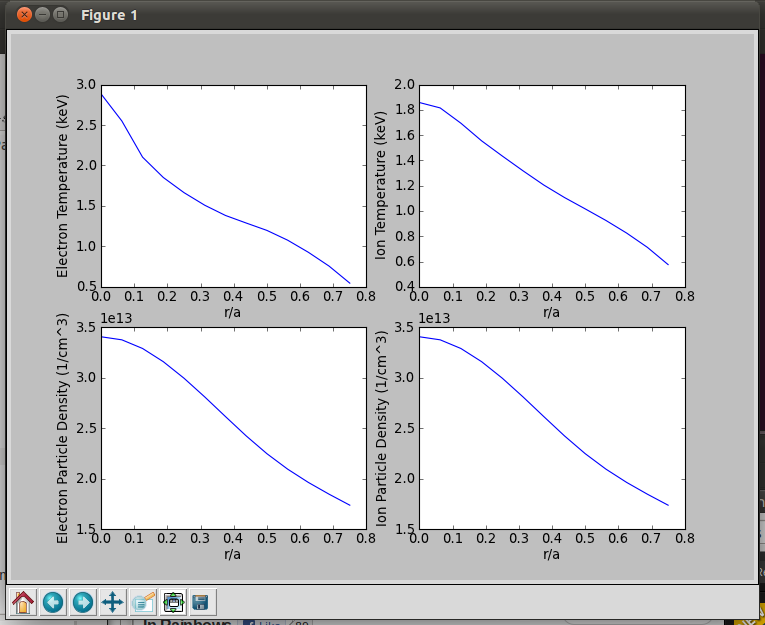
\includegraphics[scale=.5]{pssht1.png}
  \caption{Summary plots for an example TGYRO simulation.}
\end{figure}

\subsection{Command Line Use}
\noindent This functionality is also available from the terminal command line (as opposed to the python interpreter) with the simple command:

\fontfamily{\ttdefault}\selectfont

\$ tgyro\_plot -p ps

\fontfamily{\rmdefault}\selectfont

\noindent When executed from the treg01 directory, the above command produces almost the same plot:

\begin{figure}[H]
  \centering
    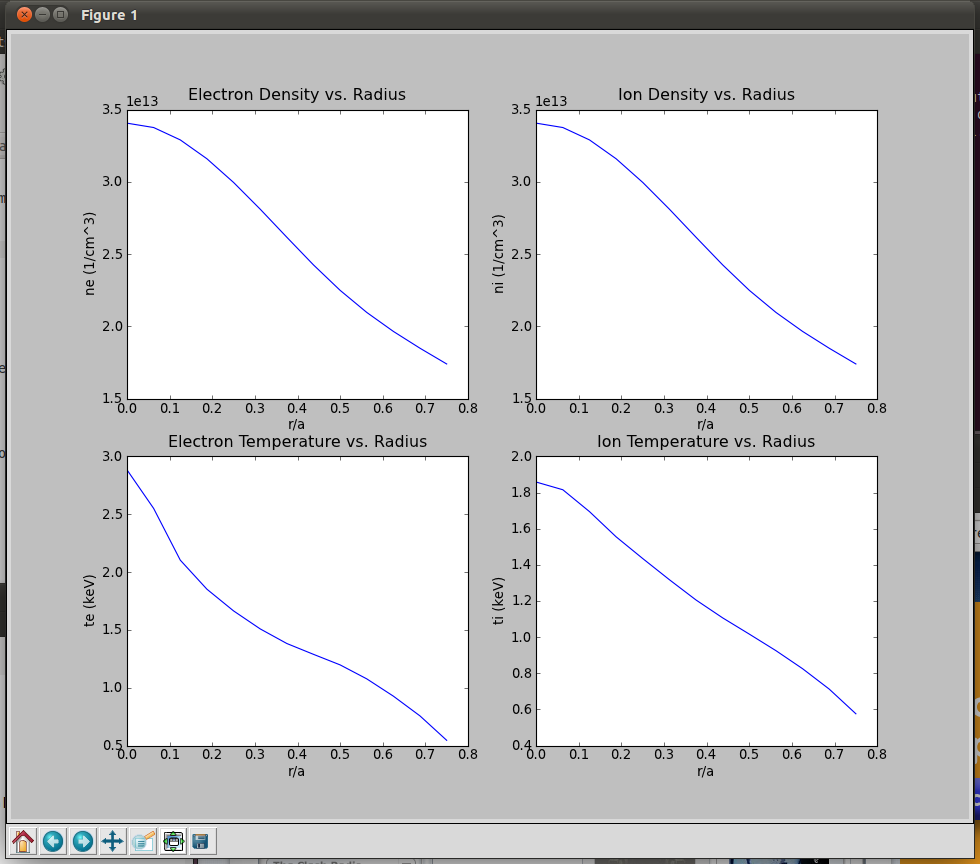
\includegraphics[scale=.35]{pssht2.png}
  \caption{Summary plots for an example TGYRO simulation produced with command line tools.}
\end{figure}

\subsection{Help Files}
\noindent The rest of this document is documentation for the classes that make up PYRATS.  Each class also has an associated help file that describes the contents of the different data containers in more detail.  The help for each code (GYRO, NEO, and TGYRO) can be accessed from the corresponding PYRATS subfolder in the gacode structure, like so:
\begin{verbatim}
~$ cd gacode/shared/python/pyrats
~gacode/shared/python/pyrats$ ls
build  examples.py   fileupload.pyx  gyro         __init__.pyc  profiles_gen  tgyro
doc    fileupload.c  fileupload.so   __init__.py  neo           setup.py
~gacode/shared/python/pyrats$ cd tgyro
~gacode/shared/python/pyrats/tgyro$ ls
data.py  data.pyc  help.py  __init__.py  __init__.pyc  interpreter.py
~gacode/shared/python/pyrats/tgyro$ python help.py ~/treg01 data
\end{verbatim}
\noindent If there is a folder named treg01 in the home directory, this command will print out all of the variables stored in the "data" container.



\newpage

\section{profiles\_genData Contents}
\subsection{Data}
\begin{itemize}
\item \textbf{data} \emph{dictionary of numpy arrays} - Contains all of the data read in by profiles\_genData.  It is organized in a dictionary with the keys being the different column headers in the input.profiles file that is read.  The keys for the dictionary can be requested with the following commands:
\fontfamily{\ttdefault}\selectfont

\$ python

>>> from pyrats.profiles\_gen.data import profiles\_genData

>>> sim1 = profiles\_genData('example\_directory')

>>> sim1.data.keys()

\fontfamily{\rmdefault}\selectfont
\noindent where, again, 'example\_directory' is a directory containing the file input.profiles.
\item \textbf{n\_exp} \emph{int} - The number of timesteps in the simulation.  It is also the length of each array in data.
\item \textbf{hlen} \emph{int} - The length of the header of file input.profiles in rows.
\item \textbf{fignum} \emph{int} - The number of the current active matplotlib figure.
\item \textbf{plotcounter} \emph{int} - The number of the current active axes on the current active matplotlib figure.
\item \textbf{ar} \emph{nested list of floats} - The sine coefficients for the r-component of the fourier series representation of the flux surfaces.  Read from input.profiles.geo.
\item \textbf{br} \emph{nested list of floats} - The cosine coefficients for the r-component of the fourier series representation of the flux surfaces.  Read from input.profiles.geo.
\item \textbf{az} \emph{nested list of floats} - The sine coefficients for the z-component of the fourier series representation of the flux surfaces.  Read from input.profiles.geo.
\item \textbf{bz} \emph{nested list of floats} - The cosine coefficients for the z-component of the fourier series representation of the flux surfaces.  Read from input.profiles.geo.
\item \textbf{directory\_name} \emph{str} - The name of the directory containing file input.profiles and possibly input.profiles.geo.
\end{itemize}
\subsection{Methods}
\begin{itemize}
\item \textbf{\_\_init\_\_(}\emph{str}\textbf{ directory='.')} - This is the constructor for the class.  When a new instance of the class is created, the constructor is called and executed.  The only argument is the name of the directory from which to build the class, and it defaults to the current directory.  It calls these methods in the following order:
\begin{enumerate}
\item set\_directory(\emph{str} directory)
\item init\_data()
\item store\_data()
\end{enumerate}
\item \textbf{compplot(}\emph{float}\textbf{ inner, }\emph{float}\textbf{ outer, }\emph{int}\textbf{ n, }\emph{bool}\textbf{ verbose)} - This method creates overlaid flux surface plots using both the fourier series decomposition method and the shaped Grad-Shafranov Miller-type equilibrium for the flux surfaces.
\begin{itemize}
\item Inner specifies the innermost flux surface to be plotted
\item outer specifies the outermost flux surface to be plotted
\item n specifies the number of flux surfaces to plot in between inner and outer
\item if verbose is True, the legend will display the location of each flux surface
\end{itemize}
\item \textbf{compute\_fouriereq(}\emph{float}\textbf{ r)} - This method calculates the flux surface at radius r according to the general Grad-Shafranov Fourier-series equilibrium.
\item \textbf{compute\_mtypeeq(}\emph{float}\textbf{ r)} - This method calculates the flux surface at radius r according to the shaped Grad-Shafranov Miller-type equilibrium.
\item \textbf{fourierplot(}\emph{float}\textbf{ inner, }\emph{float}\textbf{ outer, }\emph{int}\textbf{ n, }\emph{bool}\textbf{ verbose)} - This method creates flux surface plots using only the fourier series decomposition method for the flux surfaces.
\begin{itemize}
\item inner specifies the innermost flux surface to be plotted
\item outer specifies the outermost flux surface to be plotted
\item n specifies the number of flux surfaces to plot in between inner and outer
\item if verbose is True, the legend will display the location of each flux surface
\end{itemize}
\item \textbf{get(}\emph{str}\textbf{ var)} - This method returns the numpy array corresponding to var.
\item \textbf{init\_data()} - This method initializes all of the data objects.
\item \textbf{match(}\emph{float}\textbf{ val, }\emph{list}\textbf{ vec)} - This method finds the closest match to val in a \emph{list} of values (vec) and returns the index of that value.
\item \textbf{millerplot(}\emph{float}\textbf{ inner, }\emph{float}\textbf{ outer, }\emph{int}\textbf{ n, }\emph{bool}\textbf{ verbose)} - This method creates flux surface plots using only the shaped Grad-Shafranov Miller-type equilibrium for the flux surfaces.
\begin{itemize}
\item inner specifies the innermost flux surface to be plotted
\item outer specifies the outermost flux surface to be plotted
\item n specifies the number of flux surfaces to plot in between inner and outer
\item if verbose is True, the legend will display the location of each flux surface.
\end{itemize}
\item \textbf{plot(}\emph{str}\textbf{ var, }\emph{int}\textbf{ n1=2, }\emph{int}\textbf{ n2=2, }\emph{int}\textbf{ plotcounter=0, }\emph{int}\textbf{ fignum=0)} - This method creates plots of the requested data (var) using matplotlib.
\begin{itemize}
\item n1 is the horizontal number of plots in one window
\item n2 is the vertical number of plots in one window
\item plotcounter is the position on which the new graph is to be placed
\item fignum is the number of the matplotlib figure on which to place the new graph
\end{itemize}
\item \textbf{read\_data()} - This method reads in data from input.profiles.  It returns a dictionary containing the data that was read in.
\item \textbf{read\_fourier()} - This method reads in data from input.profiles.geo, and stores that data in the class objects ar, br, az, and bz.
\item \textbf{set\_directory(}\emph{str}\textbf{ directory)} - This method sets the class attribute directory\_name to directory.
\item \textbf{store\_data()} - This method reads data and renames it appropriately.  It is necessary because the names of the differetn parameters are not uniformly formatted.  store\_data cleans them up by inserting spaces where necessary, and by deleting \#-signs when necessary.
\end{itemize}

\newpage

\section{NEO Related Classes}

\subsection{NEOObject Contents}
\subsubsection{Data}
\begin{itemize}
\item \textbf{data} \emph{dictionary} - Holds the data associated with the object.
\item \textbf{units} \emph{str} - Describes the units of the data.
\item \textbf{descriptor} \emph{str} - Provides a description of the data.
\end{itemize}
\subsubsection{Methods}
\begin{itemize}
\item \textbf{\_\_init\_\_(}\emph{dict}\textbf{ data,}\emph{ str}\textbf{ units,}\emph{ str}\textbf{ descriptor)} - This method stores the appropriate arguments in the appropriate containers.
\end{itemize}

\subsection{NEOData Contents}
\subsubsection{Data}
\begin{itemize}
\item \textbf{master} \emph{str} - Holds the name of the master directory containing NEO output files.
\item \textbf{directory\_name} \emph{str} - Holds the name of the currently open directory.
\item \textbf{fignum} \emph{int} - The number of the current active matplotlib figure.
\item \textbf{plotcounter} \emph{int} - The number of the current active axes on the current active matplotlib figure.
\item \textbf{toplot} \emph{list} - The list of variables to plot when a plot command is called.
\item \textbf{transport} \emph{dictionary of dictionaries of NEOObjects} - Contains data read in from out.neo.transport.  The keys are the transport variables, each of which correspond to a NEOObject.
\item \textbf{HH\_theory} \emph{dictionary of dictionaries of NEOObjects} - Contains data read in from out.neo.theory.  The keys are the flows and fluxes predicted by the Hinton-Hazeltine model, each of which correspond to a NEOObject.
\item \textbf{CH\_theory} \emph{dictionary of dictionaries of NEOObjects} - Contains data read in from out.neo.theory.  The keys are the ion heat fluxes predicted by the Chang-Hinton model, each of which correspond to a NEOObject.
\item \textbf{TG\_theory} \emph{dictionary of dictionaries of NEOObjects} - Contains data read in from out.neo.theory.  The keys are the ion heat fluxes predicted by the Taguchi model, each of which correspond to a NEOObject.
\item \textbf{S\_theory} \emph{dictionary of dictionaries of NEOObjects} - Contains data read in from out.neo.theory. The keys are the bootstrap currents predicted by the Sauter model, each of which correspond to a NEOObject.
\item \textbf{HS\_theory} \emph{dictionary of dictionaries of NEOObjects} - Contains data read in from out.neo.theory.  The keys are the fluxes predicted by the Hirshman-Sigmar model, each of which  correspond to a NEOObject.
\item \textbf{control} \emph{dictionary of dictionaries of NEOObjects} - Contains data read in from out.neo.control.
\end{itemize}
\subsubsection{Methods}
\begin{itemize}
\item \textbf{\_\_init\_\_(}\emph{str} \textbf{sim\_directory)} - Constructor that is executed when a new NEOData object is created.  It takes a directory name as its argument, and then executes a top down walk down that directory.  It then calls read\_data() whenever it is in a subdirectory with NEO output files.  Finally, it executes store\_data()
\item \textbf{get\_input(}\emph{str} \textbf{input\_name)} - Returns requested variable from input.neo.gen.
\item \textbf{init\_data()} - Initializes object data.
\item \textbf{plot(}\emph{str} \textbf{var, }\emph{int} \textbf{n1=2, }\emph{int} \textbf{n2=2,} \emph{int} \textbf{plotcounter=0,} \emph{int} \textbf{fignum=0,} \emph{bool} \textbf{legend=True,} \emph{bool} \textbf{verbose=False,} \emph{str} \textbf{cols='bgkcmyrw',} \emph{list of strs} \textbf{styles=['-', '--', '-.', ':'])} - Plots var as a matplotlib scatter plot with data from different directories coming in different colors, and different species coming in different line styles.  Automatically searches for both theoretical and simulated values, and plots everything that is available.
\item \textbf{print\_vars()} - Prints all available simulated variables.
\item \textbf{read\_data()} - Read in object data.  Calls read\_grid(), read\_equil(), read\_theory(), read\_transport(), read\_transport\_gv().
\item \textbf{read\_equil()} - Reads out.neo.equil.  The data is eventually stored by store\_data() in control.
\item \textbf{read\_file()} - Loads data from NEO output file into buffer for manipulation and storage.
\item \textbf{read\_grid()} - Reads out.neo.grid.  The data is eventually stored by store\_data() in control.
\item \textbf{read\_theory()} - Reads out.neo.theory.  The data is eventually stored by store\_data() in HH\_theory, TG\_theory, CH\_theory, S\_theory, HR\_theory, and HS\_theory.
\item \textbf{read\_transport()} - Reads out.neo.transport.  The data is eventually stored by store\_data() in transport.
\item \textbf{read\_transport\_gv()} - Reads out.neo.transport\_gv.  The data is eventually stored by store\_data() in transport.
\item \textbf{set\_directory(}\emph{str} \textbf{path)} - Sets the current directory to path.
\item \textbf{split(}\emph{list} \textbf{array)} - Takes a 2-D list which has entries with multiple elements and converts it to a 2-D list with only one element per entry.
\item \textbf{store\_data()} - Stores data into data dictionaries by variable name and directory.  Data can be accessed with two dictionary keys, like so:

sim1.transport[parameter][directory].
\end{itemize}

\newpage
\section{TGYROData Contents}
\subsection{Data}
\begin{itemize}
\item \textbf{loc\_n\_ion} \emph{int} - Number of ions in simulation.
\item \textbf{tgyro\_mode} \emph{int} - Mode number of TGYRO operation.
\item \textbf{n\_iterations} \emph{int} - Number of TGYRO iterations in simulation.
\item \textbf{n\_fields} \emph{int} - Number of fields in simulation.
\item \textbf{n\_radial} \emph{int} - Number of radial gridpoints in simulation.
\item \textbf{directory\_name} \emph{str} - Name of loaded directory.
\item \textbf{data} \emph{dictionary of lists of numpy arrays} - Large dictionary containing all loaded data by variable name and then by iteration number.
\end{itemize}
\subsection{Methods}
\begin{itemize}
\item \textbf{\_\_init\_\_(}\emph{str} \textbf{ sim\_directory)} - Constructor which is called when a new TRYGOData object is created.  It calls the following methods:
\begin{enumerate}
\item set\_directory(\emph{str} sim\_directory)
\item init\_data()
\item read\_data()
\end{enumerate}
\item \textbf{get\_input(}\emph{str}\textbf{ input\_name)} - Returns the specified variable from input.tgyro.gen.

Ex: get\_input("TGYRO\_MODE")
\item \textbf{get\_local\_res(}\emph{int}\textbf{ field=1,}\emph{ int}\textbf{ iteration=-1)} - Returns a numpy array of the local field residual for the given field and iteration.  The default is the last iteration, and field 1.
\item \textbf{get\_stability\_at\_radius(}\emph{int}\textbf{ radius=0,}\emph{ str}\textbf{ frequency='r',}\emph{ str}\textbf{ direction='ion')} - Returns a list of frequency vs. ky at specified radius from stability analysis.  The parameter radius is the requested radial index; it is an integer between 0 and n\_r-1.  The parameter frequency can be either the real ('r') or the imaginary ('i') spectrum.  The parameter direction specifies the direction of the spectrum.  It can be either the ion direction ('ion') or the electron direction ('elec').
\item \textbf{init\_data()} - Initializes object data.
\item \textbf{make\_gradient\_vs\_field\_plot(}\emph{int}\textbf{ r=1,}\emph{ int}\textbf{ evolve\_field=1,}\emph{ str}\textbf{ grad='a/LTi',}\emph{ str}\textbf{ profile='ti',}\emph{ bool}\textbf{ arrows=False)} - Return a matplotlib.pyplot figure of gradient\_vs\_field\_space.  The parameter r is the radial index; it is an integer between 0 and n\_r-1.  The parameters are passed to make\_gradient\_vs\_field\_space, and are described there.
\item \textbf{make\_gradient\_vs\_field\_space(}\emph{int}\textbf{ r=1,}\emph{ int}\textbf{ evolve\_field=1,}\emph{ str}\textbf{ grad='a/LTi',}\emph{ str}\textbf{ profile='ti')} - Returns a matrix of Space[iteration][gradient,profile,residual] at givel radial point.  eeg: Space[[4.0, 1.7, 2.5], [3.6, 1.5, 0.1]] if grad 4.0 $\rightarrow$ 3.6 while Ti $\rightarrow$ 1.5 and local residual went from 2.5 $\rightarrow$ 0.1.  The parameter evolve\_field specifies the field type to pass to get\_local\_res.  The parameter grad is the gradient factor to pass to get\_gradient\_factor.  The parameter profile is the profile factor to pass to get\_profile\_factor.
\item \textbf{read\_chi\_e()} - Internal method.  This method reads in chi\_e.out and stores it in self.chi\_e.
\item \textbf{read\_chi\_i()} - Internal method.  This method reads in chi\_i.out and stores it in self.chi\_i.
\item \textbf{read\_control()} - Internal method.  This method reads in control.out to set resolutions.
\item \textbf{read\_data()} - Internal method.  This method reads in object data and calls the following other methods:
\begin{enumerate}
\item read\_control()
\item read\_chi\_e()
\item read\_chi\_i(loc\_n\_ion)
\item read\_gyrobohm()
\item read\_profile()
\item read\_geometry()
\item read\_flux(loc\_n\_ion)
\item read\_mflux(loc\_n\_ion)
\item read\_gradient()
\item read\_residual()
\end{enumerate}
\item \textbf{read\_file(}\emph{str}\textbf{ file\_name)} - Reads TGYRO output file.  Output is data['column\_header'][iteration]
\item \textbf{read\_flux(}\emph{int}\textbf{ num\_ions=1)} - Reads flux\_e.out, flux\_i(2-5).out, and flux\_target.out.  Num\_ions determines how many ion files to read.
\item \textbf{read\_geometry()} - Reads and stores geometry.out in self.geometry.
\item \textbf{read\_gradient()} - Reads and stores gradient.out in self.gradient.
\item \textbf{read\_gyrobohm()} - Reads and stores gyrobohm.out in self.gyro\_bohm\_unit.
\item \textbf{read\_mflux()} - Reads and stores mflux\_e.out, mflux\_i(2-5).out, and mflux\_target.out.
\item \textbf{read\_num\_ions()} - Reads LOC\_N\_ION and stores it as self.loc\_n\_ion.
\item \textbf{read\_profile()} - Reads and stores profile.out in self.profile.
\item \textbf{read\_profile2()} - Reads and stores profile2.out in self.profile2.
\item \textbf{read\_profile3()} - Reads and stores profile3.out in self.profile3.
\item \textbf{read\_profile4()} - Reads and stores profile4.out in self.profile4.
\item \textbf{read\_profile5()} - Reads and stores profile5.out in self.profile5.
\item \textbf{read\_residual()} - Reads residual.out.
\item \textbf{read\_stab\_file(}\emph{str}\textbf{ file\_name)} - Reads files generated with stability analysis mode.  The parameter file\_name is the name of the requested stability file, sich as "wi\_elec.out".  It returns a list of [r, ks, freq].
\item \textbf{read\_stabilities()} - Reads output files from TGYRO\_METHOD=2, and stores them into variables, as follows:
\begin{itemize}
\item wr\_ion.out $\rightarrow$ self.wr\_ion
\item wi\_ion.out $\rightarrow$ self.wi\_ion
\item wr\_elec.out $\rightarrow$ self.wr\_elec
\item wi\_elec.out $\rightarrow$ self.wi\_elec
\end{itemize}
\item \textbf{read\_tgyro\_mode()} - Reads the TGYRO\_MODE and stores it as self.tgyro\_mode.
\item \textbf{set\_directory(}\emph{str}\textbf{ sim\_directory)} - Sets the simulation directory.  Stores sim\_directory in

self.directory\_name.
\end{itemize}

\newpage
\section{GYROData Contents}
\subsection{Data}
\begin{itemize}
\item \textbf{directory\_name}\emph{ str} - The name of the simulation directory.
\item \textbf{profile}\emph{ dictionary of numpy arrays} - Dictionary where control information from out.gyro.profile is stored.  The keys can be obtained by typing: sim1.profile.keys()
\item \textbf{geometry}\emph{ dictionary of numpy arrays} - Dictionary where geometry data from out.gyro.geometry is stored.  The keys can be obtained by typing: sim1.geometry.keys()
\item \textbf{t}\emph{ dictionary of numpy arrays} - Dictionary where time data from t.out is stored.  The keys are: 't/deltat', '(cbar\_s/a)t', and 'n\_time' which is an int, not a numpy array.
\item \textbf{diff}\emph{ numpy array} - Numpy array with dimensions of (n\_kinetic, n\_field, moments=2, n\_time).  It contains the Gyrobohm-normalized diffusivities averaged over radius and summer over mode number.  The moments are:
\begin{enumerate}
\item $D_\sigma/\chi_{GB}$ (particle diffusivity)
\item $\chi_\sigma/\chi_{GB}$ (energy diffusivity)
\end{enumerate}
\item \textbf{diff\_i}\emph{ numpy array} - Numpy array with dimensions of (n\_kinetic, n\_field, moments=2, n\_x, n\_time).  It contains the Gyrobohm-normalized diffusivities as a function of radius, summed over mode number.  The moments are:
\begin{enumerate}
\item $D_\sigma(r)/\chi_{GB}$ (particle diffusivity)
\item $\chi_\sigma(r)/\chi_{GB}$ (energy diffusivity)
\end{enumerate}
\item \textbf{diff\_n}\emph{ numpy array} - Numpy array with dimensions of (n\_kinetic, n\_field, moments=2, n\_n, n\_time).  It contains the Gyrobohm-normalized diffusivities averaged over radius for each mode number.  The moments are:
\begin{enumerate}
\item $D_{\sigma,n}/\chi_{GB}$ (particle diffusivity)
\item $\chi_{\sigma,n}/\chi_{GB}$ (energy diffusivity)
\end{enumerate}
\item \textbf{gbflux}\emph{ numpy array} - Numpy array with dimensions of (n\_kinetic, n\_field, moments=4, n\_time).  It contains the Gyrobohm-normalized fluxes averaged over radius and summed over mode number.  The moments are:
\begin{enumerate}
\item $\Gamma_\sigma/\Gamma_{GB}$ (particle flux)
\item $Q_\sigma/Q_{GB}$ (energy flux)
\item $\Pi_\sigma/\Pi_{GB}$ (momentum flux)
\item $S^{tur}_{W,\sigma}/S_{GB}$ (exchange power density)
\end{enumerate}
\item \textbf{gbflux\_i}\emph{ numpy array} - Numpy array with dimensions of (n\_kinetic, n\_field, moments=4, n\_x, n\_time).  It contains the Gyrobohm-normalized fluxes as a function of mode number and averaged over radius.  The moments are:
\begin{enumerate}
\item $\Gamma_\sigma(r)/\Gamma_{GB}$ (particle flux)
\item $Q_\sigma(r)/Q_{GB}$ (energy flux)
\item $\Pi_\sigma(r)/\Pi_{GB}$ (momentum flux)
\item $S^{tur}_{W,\sigma}(r)/S_{GB}$ (exchange power density)
\end{enumerate}
\item \textbf{gbflux\_n}\emph{ numpy array} - Numpy array with dimensions of (n\_kinetic, n\_field, moments=4, n\_n, n\_time).  It contains the Gyrobohm-normalized fluxes as a function of mode number and averaged over radius.  The moments are:
\begin{enumerate}
\item $\Gamma_\sigma/\Gamma_{GB}$ (particle flux)
\item $Q_\sigma/Q_{GB}$ (energy flux)
\item $\Pi_\sigma/\Pi_{GB}$ (momentum flux)
\item $S^{tur}_{W,\sigma}/S_{GB}$ (exchange power density)
\end{enumerate}
\item \textbf{moment\_u}\emph{ numpy array} - Complex numpy array with dimensions of (n\_theta\_plot, n\_x, i\_field=n\_field, n\_n, n\_time).  It contains the potential expansion coefficients.  More information is available online at https://fusion.gat.com/theory/Gyrousermanual\#Computed\_Quantities.  The fields are described below.  There can be up to three different fields:
\begin{enumerate}
\item $\frac{e\delta\phi_n}{\bar{T}_e}$ (electrostatic potential)
\item $\frac{\bar{c}_s}{c}\frac{e\delta A_{\parallel n}}{\bar{T}_e}$ (electromagnetic potential)
\item $\frac{\delta B_\parallel}{B_{\mathrm{unit}}(r)}$ (compressional perturbation)
\end{enumerate}
\item \textbf{moment\_n}\emph{ numpy array} - Complex numpy array with dimensions of (n\_theta\_plot, n\_x, n\_kinetic, n\_n, n\_time).  It contains the density moment expansion coefficients: $\frac{\delta n_{\sigma,n}}{\bar{n}_e}$.  More information is available online at https://fusion.gat.com/theory/Gyrousermanual\#Computed\_Quantities.
\item \textbf{moment\_e}\emph{ numpy array} - Complex numpy array with dimensions of (n\_theta\_plot, n\_x, n\_kinetic, n\_n, n\_time).  It contains the energy moment expansion coefficients: $\frac{\delta E_{\sigma,n}}{\bar{n}_e\bar{T}_e}$.  More information is available online at https://fusion.gat.com/theory/Gyrousermanual\#Computed\_Quantities.
\item \textbf{moment\_v}\emph{ numpy array} - Complex numpy array with dimensions of (n\_theta\_plot, n\_x, n\_kinetic, n\_n, n\_time).  It contains the parallel velocity moment expansion coefficients: $\frac{\delta V_{\sigma,n}}{\bar{n}_e\bar{c}_s}$.  More information is available online at https://fusion.gat.com/theory/Gyrousermanual\#Computed\_Quantities.
\item \textbf{moment\_zero}\emph{ numpy array} - Numpy array with dimensions of (n\_x, n\_kinetic, moments=n\_moment, n\_time).  It contains the flux-surface average of the $n=0$ component of the density and energy moments.  The moments are described below.  There can be up to two different moments:
\begin{enumerate}
\item $\langle\frac{\delta n_{\sigma,0}}{\bar{n}_e}\rangle$
\item $\langle\frac{\delta E_{\sigma,0}}{\bar{n}_e\bar{T}_e}\rangle$
\end{enumerate}
\item \textbf{flux\_velocity}\emph{ numpy array} - Numpy array with dimensions of (n\_energy, n\_lambda, n\_kinetic, i\_field=n\_field, moments=2, n\_n, n\_time).  It contains the velocity-space flux densities: $$\Gamma=\int \! \dif \varepsilon \int \! \dif \lambda \, \Gamma(\varepsilon, \lambda), \, \, \, \, Q=\int \! \dif \varepsilon \int \! \dif \lambda \, Q(\varepsilon, \lambda)$$
The moments are:
\begin{enumerate}
\item $\Gamma{\sigma,n}(\varepsilon,\lambda)$ (particle flux)
\item $Q_{\sigma,n}(\varepsilon,\lambda)$ (energy flux)
\end{enumerate}
The possible fields are:
\begin{enumerate}
\item electrostatic component
\item electromagnetic component
\end{enumerate}
\item \textbf{k\_perp\_squared}\emph{ numpy array} - Numpy array with dimensions of (n\_n, n\_time).  It contains the flux-surface and radial average of $k^2_\perp$:
$$\frac{\langle\langle(k_\perp\bar{\rho}_{s,\mathrm{unit}})^2|\delta\phi_n|^2\rangle\rangle_r}{\langle\langle|\delta\phi_n|^2\rangle\rangle_r}$$
\end{itemize}
\subsection{Methods}
\begin{itemize}
\item \textbf{\_\_init\_\_(}\emph{str}\textbf{ sim\_directory)} - This is the class constructor.  It is called when a new object of that class is created, and it reads in data from sim\_directory to create that object.  It sets the variable directory\_name to sim\_directory, and appends the pyrats folder to the python search path.  It also calls the following methods:
\begin{enumerate}
\item init\_data()
\item read\_data()
\item equil\_time()
\end{enumerate}
\item \textbf{equil\_time()} - This method counts the number of time steps present in the currently loaded arrays, and sets them all equal (to the length of the array with the fewest number of time steps).
\item \textbf{get\_input(}\emph{str}\textbf{ input\_name)} - This method returns the specified variable from input.gyro.gen.  Ex: get\_input("TIME\_STEP")
\item \textbf{init\_data()} - This method initializes object data.
\item \textbf{make\_diff()} - This method creates self.diff by computing it from self.gbflux.
\item \textbf{make\_diff\_i()} - This method creates self.diff\_i by computing it from self.gbflux\_i.
\item \textbf{make\_gbflux()} - This method creates self.gbflux by averaging over the radial component of self.gbflux\_i.
\item \textbf{plot(}\emph{list}\textbf{ x,}\emph{ list}\textbf{ y,}\emph{ tuple}\textbf{ dim=(1, 1))} - This method creates a matplotlib plot of the requested data.
\item \textbf{read\_data()} - This method reads in object data.  It executes:
\begin{enumerate}
\item read\_profile()
\item read\_geometry()
\item read\_t()
\item read\_gbflux\_i()
\item read\_gbflux\_n()
\end{enumerate}
\item \textbf{read\_file(}\emph{str}\textbf{ fname,}\emph{ int}\textbf{ dSize)} - This method reads the GYRO data file named out.gyro.fname.  It must be given the length in number of characters of the data elements in the file as a second argument.
\item \textbf{read\_flux\_velocity()} - This method reads in flux\_velocity data, and stores it in self.flux\_velocity.
\item \textbf{read\_freq()} - This method reads in frequency data and stores it in self.freq.
\item \textbf{read\_gbflux\_i()} - This method reads in gbflux\_i data and stores it in self.gbflux\_i.
\item \textbf{read\_gbflux\_n()} - This method reads in gbflux\_n data and stores it in self.gbflux\_n.
\item \textbf{read\_geometry()} - This method reads in geometry\_array data and stores it in self.geometry.
\item \textbf{read\_k\_perp\_squared()} - This method reads in k\_perp\_squared data and stores it in self.k\_perp\_squared.
\item \textbf{read\_moment\_e()} - This method reads in moment\_e data and stores it in self.moment\_e.
\item \textbf{read\_moment\_n()} - This method reads in moment\_n data and stores it in self.moment\_n.
\item \textbf{read\_moment\_u()} - This method reads in moment\_u data and stores it in self.moment\_u.
\item \textbf{read\_moment\_v()} - This method reads in moment\_v data and stores it in self.moment\_v.
\item \textbf{read\_moment\_zero()} - This method reads in moment\_zero data and stores it in self.moment\_zero.
\item \textbf{read\_profile()} - This method reads out.gyro.profile to get control data and stores it in self.profile.
\item \textbf{read\_t()} - This method reads t.out to get time data and stores it in self.t.
\item \textbf{set\_directory(}\emph{str}\textbf{ path)} - This method sets the variable self.directory\_name to path.
\end{itemize}
\end{document}
